\documentclass[tikz]{standalone}

\usetikzlibrary{calc}

\begin{document}
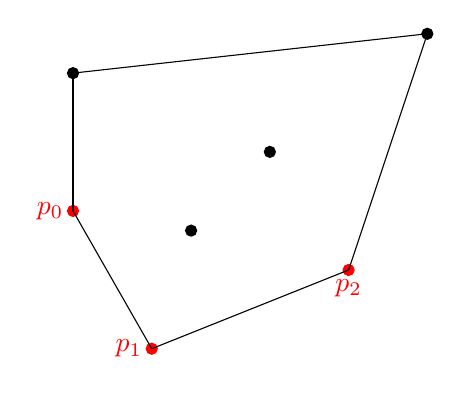
\begin{tikzpicture}

    \filldraw[black] (0.5, 0) coordinate(p0) circle (2pt) ;
    \filldraw[red] (1.5,-1.5) coordinate(p1) circle (2pt) node[below] {$p_2$} ;
    \filldraw[red] (-1,-2.5) coordinate(p2) circle (2pt) node[left] {$p_1$};
    \filldraw[black] (2.5,1.5) coordinate(p3) circle (2pt) ;
    \filldraw[black] (-2,1) coordinate(p4) circle (2pt) ;
    \filldraw[red] (-2,-0.75) coordinate(p5) circle (2pt) node[left] {$p_0$};
    \filldraw[black] (-0.5,-1) coordinate(p6) circle (2pt);
    
    \draw[black] (p5) -- (p2);
    \draw[black] (p2) -- (p1);
    \draw[black] (p1) -- (p3);
    \draw[black] (p3) -- (p4);
    \draw[black] (p4) -- (p5);
    

\end{tikzpicture}
\end{document}